%%%%%%%%%%%%%%%%%%%%%%%%%%%%%%%%%%%%%%%%%%%%%%%%%%%%%%%%%%%%%%%%%%%%%%%%%%%%%%%%
%% ************************************************************************** %%
%% *                                PREAMBLE.                               * %%
%% ************************************************************************** %%
%%%%%%%%%%%%%%%%%%%%%%%%%%%%%%%%%%%%%%%%%%%%%%%%%%%%%%%%%%%%%%%%%%%%%%%%%%%%%%%%
\documentclass[lettersize,journal]{IEEEtran}
%  \begin{list}{}{}
%    \item{Regular Journal Article}
%    \item{{\tt{$\backslash$documentclass[journal]{IEEEtran}}}}\\
%    \item{{Conference Paper}}
%    \item{{\tt{$\backslash$documentclass[conference]{IEEEtran}}}}\\
%    \item{Computer Society Journal Article}
%    \item{{\tt{$\backslash$documentclass[10pt,journal,compsoc]{IEEEtran}}}}\\
%    \item{Computer Society Conference Paper}
%    \item{{\tt{$\backslash$documentclass[conference,compsoc]{IEEEtran}}}}\\
%    \item{{Communications Society Journal Article}}
%    \item{{\tt{$\backslash$documentclass[journal,comsoc]{IEEEtran}}}}\\
%    \item{{Brief, Correspondence or Technote}}
%    \item{{\tt{$\backslash$documentclass[9pt,technote]{IEEEtran}}}}
%  \end{list}

\usepackage{amsmath,amsfonts}
\usepackage{algorithmic}
\usepackage{array}
\usepackage[caption=false,font=normalsize,labelfont=sf,textfont=sf]{subfig}
\usepackage{textcomp}
\usepackage{stfloats}
\usepackage{url}
\usepackage{verbatim}
\usepackage{graphicx}
\hyphenation{op-tical net-works semi-conduc-tor IEEE-Xplore}
\def\BibTeX{{\rm B\kern-.05em{\sc i\kern-.025em b}\kern-.08em
    T\kern-.1667em\lower.7ex\hbox{E}\kern-.125emX}}
\usepackage{balance}

%%%%%%%%%%%%%%%%%%%%%%%%%%%%%%%%%%%%%%%%%%%%%%%%%%%%%%%%%%%%%%%%%%%%%%%%%%%%%%%%
%% ************************************************************************** %%
%% *                           [JX] STYLES & CONFIG.                        * %%
%% ************************************************************************** %%
%%%%%%%%%%%%%%%%%%%%%%%%%%%%%%%%%%%%%%%%%%%%%%%%%%%%%%%%%%%%%%%%%%%%%%%%%%%%%%%%
% + [JX] add chapter functionality in article class
\usepackage[]{hyperref}
\newcounter{Chapcounter}
\newcommand\showmycounter{\addtocounter{Chapcounter}{1}\themycounter}
\newcommand{\chapter}[1] 
{ {\centering          
  \addtocounter{Chapcounter}{1} \Large \underline{\textbf{ \color{blue} Chapter \theChapcounter: ~#1}} }   
  \addcontentsline{toc}{section}{\underline{[Chapter:~\theChapcounter]~~ #1}}  
  \vspace{1em} 
}
%%%%

%% %[+JX] SI Units
\RequirePackage{siunitx}

%% %[+JX] glossaries (must be loaded after hyperref package) and style
%\RequirePackage[acronym,nonumberlist,section]{glossaries}
\RequirePackage[section]{glossaries}
\RequirePackage{glossary-tree}
\RequirePackage{glossaries-extra}
\makeglossaries
\loadglsentries{glossaries}

%% %[+JX] additional math packages
\RequirePackage{physics}
\RequirePackage{cancel}

%% %[+JX] bib
\bibliographystyle{IEEEtran}

%%%%%%%%%% %[+JX] custom styling:
% TODO Flags
\RequirePackage{xcolor}
\newcommand\TODO[1]{{\textcolor{red}{\textbf{#1}}}}
\newcommand\ATTR[1]{{\textcolor{blue}{\textbf{#1}}}}
\newcommand\COMMENT[1]{\textcolor{orange}{#1}}

%%%  Equation Condition
\newenvironment{eqconditions}
  {\par\vspace{\abovedisplayskip}\noindent\begin{tabular}{>{$}l<{$} @{${}={}$} l}}
  {\end{tabular}\par\vspace{\belowdisplayskip}}
\newenvironment{eqconditions*}
  {\noindent\begin{tabular}{>{$}l<{$} @{${}={}$} l}}
  {\end{tabular}}

% custom math command
\newcommand{\unit}[1]{\left[\si{#1}\right]}

%%%%%%%%%% %[+JX] shortcuts styling:
%% MATH %%
\newcommand{\RR}{\mathds{R}}
\newcommand{\R}{\mathbb{R}}
\newcommand{\sign}{\mathop{\mathrm{sign}}}
\newcommand{\argmin}{\mathop{\mathrm{argmin}}}
\newcommand{\zero}{\mathbf{0}}
\newcommand{\one}{\mathbf{1}}
\newcommand{\bv}{\mathbf{b}}
\newcommand{\wv}{\mathbf{w}}
\newcommand{\xv}{\mathbf{x}}
\newcommand{\av}{\mathbf{a}}
\newcommand{\yv}{\mathbf{y}}
\newcommand{\rv}{\mathbf{r}}
\newcommand{\inner}[2]{\langle #1, #2 \rangle}
\newcommand{\magenta}[1]{{\color{magenta}#1}}

\newcommand{\xspace}{\;}
\newcommand{\ea}{\textbf{et al.}\xspace}
\newcommand{\eg}{\textbf{e.g.}\xspace}
\newcommand{\ie}{\textbf{i.e.}\xspace}
\newcommand{\iid}{\textbf{i.i.d.}\xspace}
\newcommand{\cf}{\textbf{cf.}\xspace}
\newcommand{\wrt}{\textbf{w.r.t.}\xspace}
\newcommand{\aka}{\textbf{a.k.a.}\xspace}
\newcommand{\etc}{\textbf{etc.}\xspace}
\newcommand{\st}{\textbf{s.t.}\xspace}

\newcommand{\ans}[1]{{\textcolor{orange}{\textsf{Ans}: #1}}}
\newcommand{\SE}[1]{\textrm{SE(#1)}}
\newcommand{\se}[1]{\textrm{se(#1)}}
\newcommand{\SO}[1]{\textrm{SO(#1)}}
\newcommand{\so}[1]{\textrm{so(#1)}}

\newcommand{\bm}[1]{\mathbf{#1}}

% + [JX]: I am lazy shortcuts:
\newcommand{\Hz}[1]{{#1}\,[Hz] }
\newcommand{\VIO}{\gls{VIO} }
\newcommand{\VO}{\gls{VO} }
\newcommand{\SOTA}{\gls{SOTA} }
\newcommand{\SUMMIT}{\gls{Summit} }
\newcommand{\WAM}{\gls{WAM} }
\newcommand{\BHand}{\gls{BHand} }
\newcommand{\eih}{eye-in-hand }
\newcommand{\EE}{\gls{EE} }


\newcommand\mat[1]{\begin{matrix}#1\end{matrix}} 
\newcommand\pbracket[1]{\left( #1 \right)} 
\newcommand\bbracket[1]{\left[ #1 \right]} 
\newcommand{\matp}[1]{\pbracket{ \mat{ #1 } }}
\newcommand{\matb}[1]{\bbracket{ \mat{ #1 } }}

\newcommand{\I}{\mathbf{I}}

% [+JX] screw:
\newcommand{\expxi}[1]{e^{\hat\xi_{#1}\theta_{#1}}}
\newcommand{\expw}[1]{e^{\hatw_{#1}\theta_{#1}}}
\newcommand{\hatw}{\hat\omega}
%%%%%%%%%%%%%%%%%%%%%%%%%%%%%%
%% %[+JX] collections
\RequirePackage{enumitem}


% + [JX]:  fancy chapter styling --x does not work in article, using custom chapter command
%\usepackage[Lenny]{fncychap} %
%\ChNameUpperCase
%\ChNumVar{\fontsize{40}{42}\usefont{OT1}{ptm}{m}{n}\selectfont}
%\ChTitleVar{\Large\sc}% [USER] PICK Document style:

%% %[+JX] for more clever way of referencing (must be loaded after hyperref package)
\RequirePackage[nameinlink, noabbrev]{cleveref}

% + subfolder and filesd
\graphicspath{{Figs/}}
\usepackage{subfiles} % Best loaded last in the preamble

%%%%%%%%% ================================================================== %%%%%%%%%
%%%%%%%%%                     [ START OF MAIN BODY ]                         %%%%%%%%%
%%%%%%%%% ================================================================== %%%%%%%%%

%%%%%%%%%%%%%%%%%%%%%%%%%%%%%%%%%%%%%%%%%%%%%%%%%%%%%%%%%%%%%%%%%%%%%%%%%%%%%%%%
%% ************************************************************************** %%
%% *                                TEMPLATE.                               * %%
%% ************************************************************************** %%
%%%%%%%%%%%%%%%%%%%%%%%%%%%%%%%%%%%%%%%%%%%%%%%%%%%%%%%%%%%%%%%%%%%%%%%%%%%%%%%%
% %% Enumerate with reference:
%    \begin{enumerate}[label=\textbf{A.\arabic*}]
%    \item a
%    \item \label{l} b
%    \item c. goto \ref{l}
%    \end{enumerate}

%%%%%%%%%%%%%%%%%%%%%%%%%%%%%%%%%%%%%%%%%%%%%%%%%%%%%%%%%%%%%%%%%%%%%%%%%%%%%%%%
%% ************************************************************************** %%
%% *                                DOCUMENT.                               * %%
%% ************************************************************************** %%
%%%%%%%%%%%%%%%%%%%%%%%%%%%%%%%%%%%%%%%%%%%%%%%%%%%%%%%%%%%%%%%%%%%%%%%%%%%%%%%%
\begin{document}

\title{A clustered of \gls{SOTA} Paper}
\author{John Doe \thanks{University of Waterloo}}
 
\markboth{IEEE Journal, Last Edited: \today}{J. Xu}



\maketitle

% + [JX] Table of Contents:
\tableofcontents
%    \twocolumn[ 
%        \begin{@twocolumnfalse} 
%            \tableofcontents
%        \end{@twocolumnfalse} 
%    ]
%

\clearpage

%%%%%%%%%%%%%%%%%%%%%%%%%%%%%%%%%%%%%%%%%%%%%%%%%%%%%%%%%%%%%%%%%%%%%%%%%%%%%%%%
%% ************************************************************************** %%
%% *                              CHAPTER 01.                               * %%
%% ************************************************************************** %%
%%%%%%%%%%%%%%%%%%%%%%%%%%%%%%%%%%%%%%%%%%%%%%%%%%%%%%%%%%%%%%%%%%%%%%%%%%%%%%%%
\chapter{Template}

%%%%%%%%%%%%%%%%%%%%%%%%%%%%%%%%%%%%%%%%%%%%%%%%%%%%%%%%%%%%%%%%%%%%%%%%%%%%%%%%
%% ************************************************************************** %%
%% *                                ABSTRACT.                               * %%
%% ************************************************************************** %%
%%%%%%%%%%%%%%%%%%%%%%%%%%%%%%%%%%%%%%%%%%%%%%%%%%%%%%%%%%%%%%%%%%%%%%%%%%%%%%%%
\begin{abstract}
This document describes the most common article elements and how to use the IEEEtran class with \LaTeX \ to produce files that are suitable for submission to the Institute of Electrical and Electronics Engineers (IEEE).  IEEEtran can produce conference, journal and technical note (correspondence) papers with a suitable choice of class options.
\end{abstract}

\begin{IEEEkeywords}
Class, IEEEtran, \LaTeX, paper, style, template, typesetting.
\end{IEEEkeywords}


%%%%%%%%%%%%%%%%%%%%%%%%%%%%%%%%%%%%%%%%%%%%%%%%%%%%%%%%%%%%%%%%%%%%%%%%%%%%%%%%
%% ************************************************************************** %%
%% *                            I - INTRO.                                  * %%
%% ************************************************************************** %%
%%%%%%%%%%%%%%%%%%%%%%%%%%%%%%%%%%%%%%%%%%%%%%%%%%%%%%%%%%%%%%%%%%%%%%%%%%%%%%%%
\section{Introduction}
\IEEEPARstart{I}{ntroduduction} starts here

%%%%%%%%% ========== [Definitions] ========== %%%%%%%%%
\subsection{Definitions}
Here, we will define \cite{FrictionPreferredGrasp} as in \Cref{fig:1}.
%% - FIG -- BEGIN --------------- %% [
\begin{figure}[h]
    \centering
    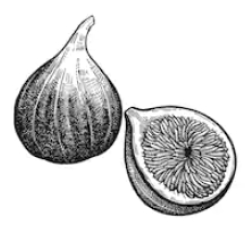
\includegraphics[width=2in]{Figs/fig1}
    \caption{A Caption}
    \label{fig:1}
\end{figure}
%% - FIG -- END ----------------- %% ]

\subsubsection{Levels}
%% - ENUM -- BEGIN --------------- %% [
\begin{enumerate}[label=\textbf{Level.\arabic*}]
    \item ABC \label{level:grasp:1}
    \item Something\label{level:grasp:2} 
    \item Repeat \label{level:grasp:3} \ref{level:grasp:2}
\end{enumerate}
%% - ENUM -- END ----------------- %% ]


%%%%%%%%%%%%%%%%%%%%%%%%%%%%%%%%%%%%%%%%%%%%%%%%%%%%%%%%%%%%%%%%%%%%%%%%%%%%%%%%
%% ************************************************************************** %%
%% *                            II - MOTIVATION                              * %%dd
%% ************************************************************************** %%
%%%%%%%%%%%%%%%%%%%%%%%%%%%%%%%%%%%%%%%%%%%%%%%%%%%%%%%%%%%%%%%%%%%%%%%%%%%%%%%%
\section{Motivation}
\noindent 


%%%%%%%%%%%%%%%%%%%%%%%%%%%%%%%%%%%%%%%%%%%%%%%%%%%%%%%%%%%%%%%%%%%%%%%%%%%%%%%%
%% ************************************************************************** %%
%% *                          III - BACKGROUND                              * %%
%% ************************************************************************** %%
%%%%%%%%%%%%%%%%%%%%%%%%%%%%%%%%%%%%%%%%%%%%%%%%%%%%%%%%%%%%%%%%%%%%%%%%%%%%%%%%
\section{Background}
\noindent \TODO{Here we will write about backgrounds}

%%%%%%%%% ========== [Visual Grasping] ========== %%%%%%%%%
\subsection{Types of visual grasping}
\TODO{surveys on different types of grasping approacches} 
\subsubsection{6-D pose grasping}
%%%%%%%%% ========== [SLAM] ========== %%%%%%%%%
\subsection{\gls{SLAM}}
\subsubsection{Kimera}

%%%%%%%%%%%%%%%%%%%%%%%%%%%%%%%%%%%%%%%%%%%%%%%%%%%%%%%%%%%%%%%%%%%%%%%%%%%%%%%%
%% ************************************************************************** %%
%% *                          IV - OUR METHODS                              * %%
%% ************************************************************************** %%
%%%%%%%%%%%%%%%%%%%%%%%%%%%%%%%%%%%%%%%%%%%%%%%%%%%%%%%%%%%%%%%%%%%%%%%%%%%%%%%%
\section{Our Methods}

%%%%%%%%% ========== [Concept] ========== %%%%%%%%%
\subsection{Conceptual Architecture}
\subsubsection{Problem Definition and Input Space}


\begin{equation}
  \hat{\xi} = \matb{\hatw & v \\ 0 & 0}, \quad 
    \hatw = \matb{\omega_1 \\ \omega_2 \\ \omega_3 }^{\wedge} = \matb{0 & -\omega_3 & \omega_2 \\ \omega_3 & 0 & -\omega_1 \\ -\omega_2 & \omega_1 & 0}
\end{equation}

%%%%%%%%%%%%%%%%%%%%%%%%%%%%%%%%%%%%%%%%%%%%%%%%%%%%%%%%%%%%%%%%%%%%%%%%%%%%%%%%
%% ************************************************************************** %%
%% *                         V - IMPLEMENTATION                             * %%
%% ************************************************************************** %%
%%%%%%%%%%%%%%%%%%%%%%%%%%%%%%%%%%%%%%%%%%%%%%%%%%%%%%%%%%%%%%%%%%%%%%%%%%%%%%%%
\section{Implementation}


\clearpage

%%%%%%%%%%%%%%%%%%%%%%%%%%%%%%%%%%%%%%%%%%%%%%%%%%%%%%%%%%%%%%%%%%%%%%%%%%%%%%%%
%% ************************************************************************** %%
%% *                              CHAPTER 02.                               * %%
%% ************************************************************************** %%
%%%%%%%%%%%%%%%%%%%%%%%%%%%%%%%%%%%%%%%%%%%%%%%%%%%%%%%%%%%%%%%%%%%%%%%%%%%%%%%%
\chapter{Template2}

%%%%%%%%%%%%%%%%%%%%%%%%%%%%%%%%%%%%%%%%%%%%%%%%%%%%%%%%%%%%%%%%%%%%%%%%%%%%%%%%
%% ************************************************************************** %%
%% *                                ABSTRACT.                               * %%
%% ************************************************************************** %%
%%%%%%%%%%%%%%%%%%%%%%%%%%%%%%%%%%%%%%%%%%%%%%%%%%%%%%%%%%%%%%%%%%%%%%%%%%%%%%%%
\begin{abstract}
This document describes the most common article elements and how to use the IEEEtran class with \LaTeX \ to produce files that are suitable for submission to the Institute of Electrical and Electronics Engineers (IEEE).  IEEEtran can produce conference, journal and technical note (correspondence) papers with a suitable choice of class options.
\end{abstract}

\begin{IEEEkeywords}
Class, IEEEtran, \LaTeX, paper, style, template, typesetting.
\end{IEEEkeywords}


%%%%%%%%%%%%%%%%%%%%%%%%%%%%%%%%%%%%%%%%%%%%%%%%%%%%%%%%%%%%%%%%%%%%%%%%%%%%%%%%
%% ************************************************************************** %%
%% *                            I - INTRO.                                  * %%
%% ************************************************************************** %%
%%%%%%%%%%%%%%%%%%%%%%%%%%%%%%%%%%%%%%%%%%%%%%%%%%%%%%%%%%%%%%%%%%%%%%%%%%%%%%%%
\section{Introduction}
\IEEEPARstart{I}{ntroduduction} starts here

%%%%%%%%% ========== [Definitions] ========== %%%%%%%%%
\subsection{Definitions}
Here, we will define \cite{FrictionPreferredGrasp} as in \Cref{fig:1}.
%% - FIG -- BEGIN --------------- %% [
\begin{figure}[h]
    \centering
    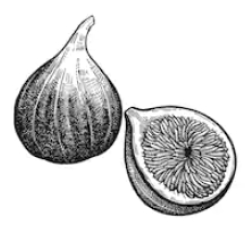
\includegraphics[width=2in]{Figs/fig1}
    \caption{A Caption}
    \label{fig:1}
\end{figure}
%% - FIG -- END ----------------- %% ]

\subsubsection{Levels}
%% - ENUM -- BEGIN --------------- %% [
\begin{enumerate}[label=\textbf{Level.\arabic*}]
    \item ABC \label{level:grasp:1}
    \item Something\label{level:grasp:2} 
    \item Repeat \label{level:grasp:3} \ref{level:grasp:2}
\end{enumerate}
%% - ENUM -- END ----------------- %% ]


%%%%%%%%%%%%%%%%%%%%%%%%%%%%%%%%%%%%%%%%%%%%%%%%%%%%%%%%%%%%%%%%%%%%%%%%%%%%%%%%
%% ************************************************************************** %%
%% *                            II - MOTIVATION                              * %%dd
%% ************************************************************************** %%
%%%%%%%%%%%%%%%%%%%%%%%%%%%%%%%%%%%%%%%%%%%%%%%%%%%%%%%%%%%%%%%%%%%%%%%%%%%%%%%%
\section{Motivation}
\noindent 


%%%%%%%%%%%%%%%%%%%%%%%%%%%%%%%%%%%%%%%%%%%%%%%%%%%%%%%%%%%%%%%%%%%%%%%%%%%%%%%%
%% ************************************************************************** %%
%% *                          III - BACKGROUND                              * %%
%% ************************************************************************** %%
%%%%%%%%%%%%%%%%%%%%%%%%%%%%%%%%%%%%%%%%%%%%%%%%%%%%%%%%%%%%%%%%%%%%%%%%%%%%%%%%
\section{Background}
\noindent \TODO{Here we will write about backgrounds}

%%%%%%%%% ========== [Visual Grasping] ========== %%%%%%%%%
\subsection{Types of visual grasping}
\TODO{surveys on different types of grasping approacches} 
\subsubsection{6-D pose grasping}
%%%%%%%%% ========== [SLAM] ========== %%%%%%%%%
\subsection{\gls{SLAM}}
\subsubsection{Kimera}

%%%%%%%%%%%%%%%%%%%%%%%%%%%%%%%%%%%%%%%%%%%%%%%%%%%%%%%%%%%%%%%%%%%%%%%%%%%%%%%%
%% ************************************************************************** %%
%% *                          IV - OUR METHODS                              * %%
%% ************************************************************************** %%
%%%%%%%%%%%%%%%%%%%%%%%%%%%%%%%%%%%%%%%%%%%%%%%%%%%%%%%%%%%%%%%%%%%%%%%%%%%%%%%%
\section{Our Methods}

%%%%%%%%% ========== [Concept] ========== %%%%%%%%%
\subsection{Conceptual Architecture}
\subsubsection{Problem Definition and Input Space}


\begin{equation}
  \hat{\xi} = \matb{\hatw & v \\ 0 & 0}, \quad 
    \hatw = \matb{\omega_1 \\ \omega_2 \\ \omega_3 }^{\wedge} = \matb{0 & -\omega_3 & \omega_2 \\ \omega_3 & 0 & -\omega_1 \\ -\omega_2 & \omega_1 & 0}
\end{equation}

%%%%%%%%%%%%%%%%%%%%%%%%%%%%%%%%%%%%%%%%%%%%%%%%%%%%%%%%%%%%%%%%%%%%%%%%%%%%%%%%
%% ************************************************************************** %%
%% *                         V - IMPLEMENTATION                             * %%
%% ************************************************************************** %%
%%%%%%%%%%%%%%%%%%%%%%%%%%%%%%%%%%%%%%%%%%%%%%%%%%%%%%%%%%%%%%%%%%%%%%%%%%%%%%%%
\section{Implementation}


\clearpage

%%%%%%%%% ================================================================== %%%%%%%%%
%%%%%%%%%                      [ END OF MAIN BODY ]                          %%%%%%%%%
%%%%%%%%% ================================================================== %%%%%%%%%
\clearpage
%%%%%%%%%%%%%%%%%%%%%%%%%%%%%%%%%%%%%%%%%%%%%%%%%%%%%%%%%%%%%%%%%%%%%%%%%%%%%%%%
%% ************************************************************************** %%
%% *                            [JX] Glossary                               * %%
%% ************************************************************************** %%
%%%%%%%%%%%%%%%%%%%%%%%%%%%%%%%%%%%%%%%%%%%%%%%%%%%%%%%%%%%%%%%%%%%%%%%%%%%%%%%%
\printglossaries    


%%%%%%%%%%%%%%%%%%%%%%%%%%%%%%%%%%%%%%%%%%%%%%%%%%%%%%%%%%%%%%%%%%%%%%%%%%%%%%%%
%% ************************************************************************** %%
%% *                             Bibliography                               * %%
%% ************************************************************************** %%
%%%%%%%%%%%%%%%%%%%%%%%%%%%%%%%%%%%%%%%%%%%%%%%%%%%%%%%%%%%%%%%%%%%%%%%%%%%%%%%%
\bibliography{[Referenced-for-report]-research}



%%%%%%%%%%%%%%%%%%%%%%%%%%%%%%%%%%%%%%%%%%%%%%%%%%%%%%%%%%%%%%%%%%%%%%%%%%%%%%%%
%% ************************************************************************** %%
%% *                                Bio.                                    * %%
%% ************************************************************************** %%
%%%%%%%%%%%%%%%%%%%%%%%%%%%%%%%%%%%%%%%%%%%%%%%%%%%%%%%%%%%%%%%%%%%%%%%%%%%%%%%%
%\begin{IEEEbiographynophoto}{Jane Doe}
%Biography text here without a photo.
%\end{IEEEbiographynophoto}
%\begin{IEEEbiography}[{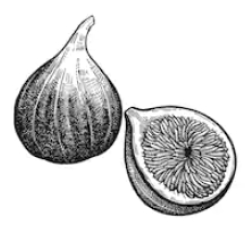
\includegraphics[width=1in,height=1.25in,clip,keepaspectratio]{Figs/fig1.png}}]{Jianxiang (Jack) Xu} 
%    University of Waterloo, MASc
%\end{IEEEbiography}

\end{document}


